\documentclass{article}
\usepackage{ctex}
\usepackage{amsmath}
\usepackage{hyperref}
\usepackage{fancyhdr}
\usepackage{graphicx}
\usepackage{subfigure}

% page settings
\topmargin=-0.45in
\evensidemargin=0in
\oddsidemargin=0in
\textwidth=6.5in
\textheight=9.0in
\headsep=0.25in
\linespread{1.1}



%配置区
\newcommand{\courseName}{Pattern Recognition}
\newcommand{\homeworkTitle}{数据聚类}
\newcommand{\studentName}{牛李金梁}%姓名
\newcommand{\studentId}{201928014629008}%学号


\newcommand{\question}[1]{\section*{Question #1}}
\renewcommand{\part}[1]{\subsection*{(#1)}}


% Header 页眉
\pagestyle{fancy}
\lhead{\studentName}
\rhead{\courseName:\homeworkTitle}
\cfoot{\thepage}

\title{
    \vspace{2in}
    %\textmd{\textbf{\courseName}:\homeworkTitle}\\
    \textmd{\textbf{\courseName}}\\
    \textmd{\homeworkTitle}\\ %cy new add
    \vspace{0.1in}
    \large{\studentName}\\
    \large{\studentId}\\
    \vspace{3in}
}

\begin{document}


\maketitle
\date{}
\pagebreak

\section*{第一部分:问题、 计算与证明}
\section*{1}
\subsection*{原理}
对混合高斯密度函数参数估计进行适当简化。
首先假设各类出现的先验概率相等。其次假设协方差矩阵是已知的。
最后假设样本的后验概率是0-1近似的,即当${\pmb{x}_k} \in w$,
$P\left( {{\omega_i}|\pmb{\pmb{x}_k},\pmb{\theta} } \right) = 1$,否则
$P\left( {{\omega_i}|\pmb{\pmb{x}_k},\pmb{\theta} } \right) = 0$。又聚类的类别数
c是已知的,所以,k-means聚类简化为混合高斯密度函数中只有
均值${\pmb{\mu} _i}$未知的情况。

根据样本到聚类中心欧氏距离的平方聚出k个类别。用最大似然估计估计
每类的均值$\pmb{\mu}  = {\left[ {{\pmb{\mu} _1}, \cdots ,{\pmb{\mu} _c}} \right]^T}$。
对每个${\pmb{\mu} _i}$似然函数为
$\ln p\left( {\pmb{x}|{\omega_i},{\pmb{\mu} _i}} \right) =  
- \ln \left( {{{\left( {2\pi } \right)}^{d/2}}{{\left| \pmb{\Sigma}  \right|}^{1/2}}} 
\right) - {1 \over 2}{\left( {\pmb{x} - {\pmb{\mu} _i}} \right)^T}{\pmb{\Sigma} ^{ - 1}}
\left( {\pmb{x} - {\pmb{\mu} _i}} \right)$。

梯度为
${\nabla _{{\pmb{\mu} _i}}}\ln p\left( {\pmb{x}|{\omega_i},{\pmb{\mu} _i}} \right)
{\rm{ = }}{\pmb{\Sigma} _i}^{ - 1}\left( {\pmb{x} - {\pmb{\mu} _i}} \right)$。

则均值${\pmb{\mu} _i}$需要满足方程:
\begin{align*}
	\sum\limits_{k = 1}^n 
	{p\left( {{\omega _i}|{x_k},\pmb{\hat \mu} } \right)} {\pmb{\Sigma} _i}^{ - 1}
	\left( {\pmb{x} - {\pmb{\hat \mu }_i}} \right) = 0,i = 1,2, \cdots, c
\end{align*}

经过整理可得
\begin{align*}
	{\pmb{\hat \mu }_i}{\rm{ = }}
	{{\sum\limits_{k = 1}^n {P\left( {{\omega _i}|{\pmb{x}_k},\pmb{\hat \mu} } \right)} {\pmb{x}_k}} 
	\over {\sum\limits_{k = 1}^n {P\left( {{\omega _i}|{\pmb{x}_k},\pmb{\hat \mu} } \right)} }} 
	= {1 \over {{n_i}}}\sum\limits_{{\pmb{x}_k} \in {\omega _i}} {{\pmb{x}_k}} ,i = 1,2 \cdots, c
\end{align*}
不过,样本${\pmb{x}_k}$属于的类别要计算到聚类中心欧氏距离的平方来判定,
因此该过程需要迭代进行。

通过迭代得到$c$个高斯成分的均值之后,一这些均值作为$c$个簇的类中心,
计算每个样本点到中心的欧式距离,将样本归入距离最近的类,从而完成一次迭代计算。

\subsection*{算法}
\begin{itemize}
	\item[1:] 设定样本个数$n$,聚类类别数$c$,
				随机初始化类中心${{\pmb{\mu} _1}, \cdots ,{\pmb{\mu} _c}}$。
	\item[2:] 对样本集进行分类。依据最近类中心原则将样本分类到某个类内。
	\item[3:] 分类后计算新的类中心${{\pmb{\mu} _1}, \cdots ,{\pmb{\mu} _c}}$。
	\item[4:] 检查迭代前后类中心是否相等,若相等则算法结束,返回类中心;
	           否则返回步骤2进行下一次迭代。  
\end{itemize}

\subsection*{影响因素}
聚类类别个数$c$对于聚类效果影响很大。

由于假设了每个类的先验概率是相等的,因此不均衡的样本、噪声较多的类和野点影响较大。

类的分布形式,如果类中心附近没有样本点,则无法聚出这一类。

\section*{2}
\subsection*{经典算法}
将样本集看成一个图结构,每个样本是图中的一个顶点,有度矩阵$\pmb{D}$。
输入亲和度矩阵$\pmb{W}$和聚类的类别数$k$
\begin{itemize}
	\item[1:] 计算图拉普拉斯矩阵$\pmb{L} = \pmb{D} - \pmb{W}$。
	\item[2:] 计算$\pmb{L}$的特征向量,选出其中前$k$小的向量
	${{\pmb{u} _1}, \cdots ,{\pmb{u} _k}}$
	组成矩阵$\pmb{U} = \left[ {{\pmb{u}_1}, \cdots ,{\pmb{u}_k}} \right] \in {R^{n \times k}}$
	\item[3:] 把$\pmb{U}$中的每一行看作1个数据点
	${\pmb{y}_i} \in {R^k},i = 1,2, \cdots ,n$
	\item[4:] 使用k-means聚类算法对${\pmb{y}_i}$聚成$k$个类别,输出这个结果。
\end{itemize}

\subsection*{Shi算法}
将样本集看成一个图结构,每个样本是图中的一个顶点,有度矩阵$\pmb{D}$。
输入亲和度矩阵$\pmb{W}$和聚类的类别数$k$
\begin{itemize}
	\item[1:] 计算图拉普拉斯矩阵$\pmb{L} = \pmb{D} - \pmb{W}$。
	\item[2:] 根据$\pmb{L}\pmb{u} = \lambda \pmb{D}\pmb{u}$
	计算随机游走型拉普拉斯矩阵${\pmb{L}_{rw}} = {\pmb{D}^{ - 1}}\pmb{L}$的特征向量,
	选出其中前$k$小的向量${{\pmb{u} _1}, \cdots ,{\pmb{u} _k}}$
	组成矩阵$\pmb{U} = \left[ {{\pmb{u}_1}, \cdots ,{\pmb{u}_k}} \right] \in {R^{n \times k}}$
	\item[3:] 把$\pmb{U}$中的每一行看作1个数据点
	${\pmb{y}_i} \in {R^k},i = 1,2, \cdots ,n$
	\item[4:] 使用k-means聚类算法对${\pmb{y}_i}$聚成$k$个类别,输出这个结果。
\end{itemize}

\subsection*{Ng算法}
将样本集看成一个图结构,每个样本是图中的一个顶点,有度矩阵$\pmb{D}$。
输入亲和度矩阵$\pmb{W}$和聚类的类别数$k$
\begin{itemize}
	\item[1:] 根据$\pmb{L} = \pmb{D} - \pmb{W}$和
	${\pmb{L}_{sym}} = {\pmb{D}^{ - 1/2}}\pmb{L}{\pmb{D}^{ - 1/2}}$
	计算对称型拉普拉斯矩阵${\pmb{L}_{sym}}$。
	\item[2:] 计算${\pmb{L}_{sym}}$的特征向量,
	选出其中前$k$小的向量${{\pmb{u} _1}, \cdots ,{\pmb{u} _k}}$
	组成矩阵
	$\pmb{U} = \left[ {{\pmb{u}_1}, \cdots ,{\pmb{u}_k}} \right] \in {R^{n \times k}}$
	\item[3:] 对$\pmb{U}$进行线性变换得到$\pmb{T} \in {R^{n \times k}}$。
	其中,${t_{ij}} = \frac{{{u_{ij}}}}{{\sqrt {\sum\nolimits_{m = 1}^n {u_{im}^2} } }}$,
	该变换使$\pmb{T}$的每行代数和为1。
	\item[4:] 把$\pmb{T}$中的每一行看作1个数据点
	${\pmb{y}_i} \in {R^k},i = 1,2, \cdots ,n$
	\item[5:] 使用k-means聚类算法对${\pmb{y}_i}$聚成$k$个类别,输出这个结果。
\end{itemize}

\subsection*{影响因素}
构建亲和力矩阵$\pmb{W}$时,$k$近邻和$\varepsilon$半径的选择会有影响。

大型矩阵的特征值分解不稳定。

进行k-means聚类的影响因素也会影响谱聚类性能。
\section*{3}
\subsection*{(1)}
${\omega _1} = \left\{ {{\pmb{x}_1},{\pmb{x}_2}} \right\}$,
${\omega _2} = \left\{ {{\pmb{x}_3},{\pmb{x}_4}} \right\}$。

类内散度矩阵${\pmb{S}_1}$、${\pmb{S}_2}$及总的类内散度矩阵${\pmb{S}_W}$为:

\begin{align*}
	{\pmb{S}_1} = \left[ {\begin{array}{*{20}{c}}
		{4.5}&{1.5}\\
		{1.5}&{0.5}
		\end{array}} \right],{\pmb{S}_2} = \left[ {\begin{array}{*{20}{c}}
		{12.5}&{-2.5}\\
		{-2.5}&{0.5}
		\end{array}} \right],{\pmb{S}_W} = \left[ {\begin{array}{*{20}{c}}
		{17}&{-1}\\
		{-1}&{1}
		\end{array}} \right]
\end{align*}

平方误差和为${J_e} = tr\left( {{\pmb{S}_W}} \right) = 18$,
类内散度矩阵行列式为$\det \left( {{\pmb{S}_W}} \right) = 16$。

\subsection*{(2)}
${\omega _1} = \left\{ {{\pmb{x}_1},{\pmb{x}_4}} \right\}$,
${\omega _2} = \left\{ {{\pmb{x}_3},{\pmb{x}_3}} \right\}$。

类内散度矩阵${\pmb{S}_1}$、${\pmb{S}_2}$及总的类内散度矩阵${\pmb{S}_W}$为:

\begin{align*}
	{\pmb{S}_1} = \left[ {\begin{array}{*{20}{c}}
		{0.5}&{-2.5}\\
		{-2.5}&{12.5}
		\end{array}} \right],{\pmb{S}_2} = \left[ {\begin{array}{*{20}{c}}
		{0.5}&{1.5}\\
		{1.5}&{4.5}
		\end{array}} \right],{\pmb{S}_W} = \left[ {\begin{array}{*{20}{c}}
		{1}&{-1}\\
		{-1}&{17}
		\end{array}} \right]
\end{align*}

平方误差和为${J_e} = tr\left( {{\pmb{S}_W}} \right) = 18$,
类内散度矩阵行列式为$\det \left( {{\pmb{S}_W}} \right) = 16$。

\subsection*{(3)}
${\omega _1} = \left\{ {{\pmb{x}_1},{\pmb{x}_2},{\pmb{x}_3}} \right\}$,
${\omega _2} = \left\{ {\pmb{x}_4} \right\}$。

类内散度矩阵${\pmb{S}_1}$、${\pmb{S}_2}$及总的类内散度矩阵${\pmb{S}_W}$为:

\begin{align*}
	{\pmb{S}_1} = \left[ {\begin{array}{*{20}{c}}
		{8.67}&{7.33}\\
		{7.33}&{8.67}
		\end{array}} \right],{\pmb{S}_2} = \left[ {\begin{array}{*{20}{c}}
		{0}&{0}\\
		{0}&{0}
		\end{array}} \right],{\pmb{S}_W} = \left[ {\begin{array}{*{20}{c}}
		{8.67}&{7.33}\\
		{7.33}&{8.67}
		\end{array}} \right]
\end{align*}

平方误差和为${J_e} = tr\left( {{\pmb{S}_W}} \right) = 17.33$,
类内散度矩阵行列式为$\det \left( {{\pmb{S}_W}} \right) = 21.33$。

通过(1)(2)(3)中的计算,可以看出:

使用平方误差和最小准则,第三种划分方式最好。

使用类内散度矩阵行列式最小准则,前两种划分方式更好。

\section*{第二部分:计算机编程}
本部分使用matlab 2019b进行编写,其他版本同样可以运行。
\section*{1}
\subsection*{(1)}
首先利用给定的代码生成了随机数组存到了文件data1.mat中,后续均采用这个数据。
具体的k-means算法可以参照第一部分的第一题。运行结果如图。
\begin{figure}[ht]
	\centering
	\subfigure{
		\begin{minipage}[t]{0.45\linewidth}
			\centering
			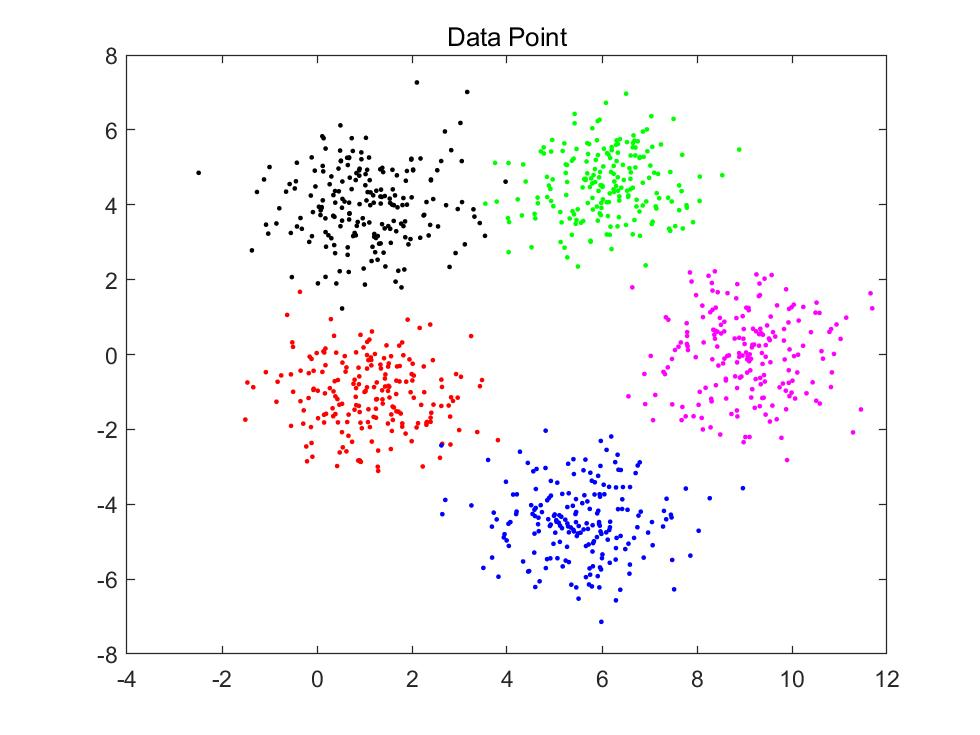
\includegraphics[width=3in]{1_1.jpg}
		\end{minipage}
	}
	\subfigure{
		\begin{minipage}[t]{0.45\linewidth}
			\centering
			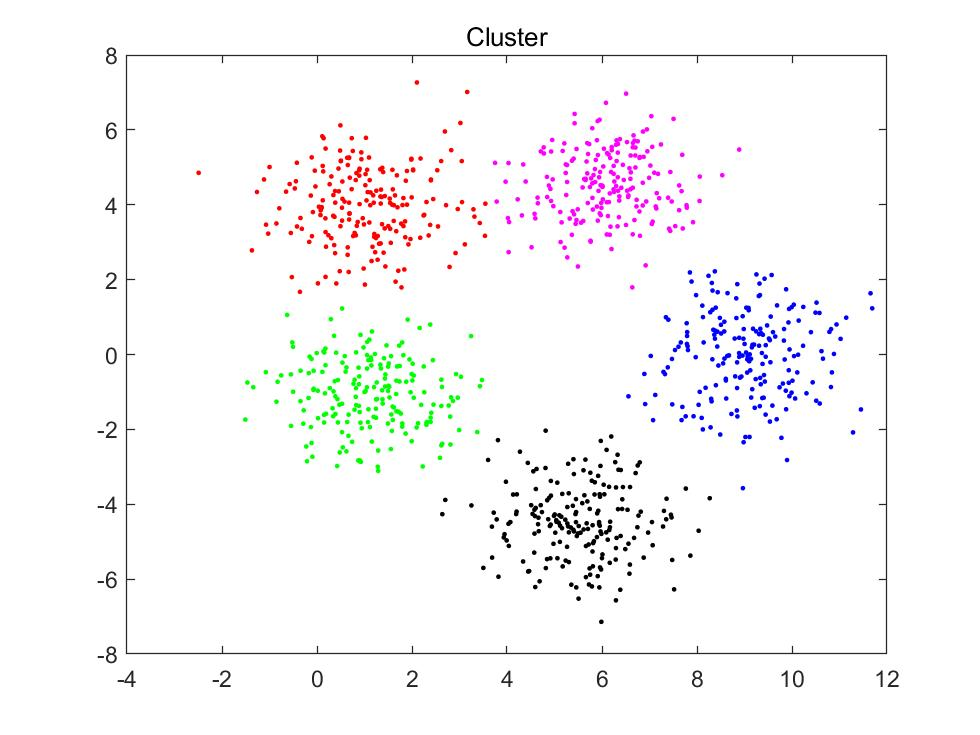
\includegraphics[width=3in]{1_2.jpg}
		\end{minipage}
	}
	\centering
	\caption{k-means算法聚类结果}
	\label{figl}
\end{figure}
\subsection*{(2)}
采用不同的初值对聚类结果差别很大,如果初始化中心周围样本很少,
将有可能得不到聚类结果。现给出一个聚类成功的结果:
\begin{itemize}
	\item 原始类中心[1, -1],聚类的类中心[1.1088,-1.0682],样本数量为200。
	\item 原始类中心[5.5, -4.5],聚类的类中心[5.5222,-4.4645],样本数量为199。
	\item 原始类中心[1, 4],聚类的类中心[1.0383,3.9929],样本数量为200。
	\item 原始类中心[6, 4.5],聚类的类中心[6.0861,4.5329],样本数量为201。
	\item 原始类中心[9, 0.0],聚类的类中心[9.0563,-0.0286],样本数量为200。
\end{itemize}

均方误差为[0.0049, 0.0016]。

\section*{2}
\subsection*{(1)}
算法参见第一部分第二题。聚类结果如图2。
\begin{figure}[ht]
	\centering
	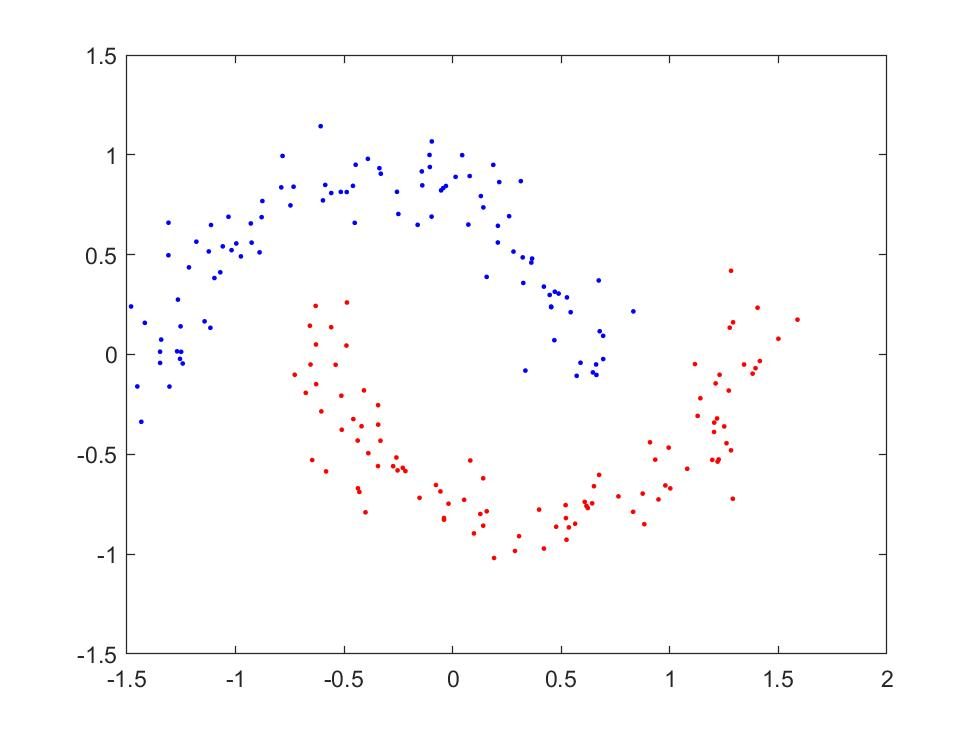
\includegraphics[width=0.5\textwidth, height = 4.8cm]{2.jpg}
	\caption{聚类结果}
	\label{figl}
\end{figure}

\subsection*{(2)}
为避免k-means算法中初始值的影响,将其固定为[-0.5, 1]和[1, -0.5]。
为测试$\sigma$对准确率的影响,将$k$固定为3,让$\sigma$以0.02步长从0.02增长到1,画出左图。
为测试$k$对准确率的影响,将$\sigma$固定为0.5,让$k$以1步长从1增长到10,画出右图。
\begin{figure}[ht]
	\centering
	\subfigure{
		\begin{minipage}[t]{0.45\linewidth}
			\centering
			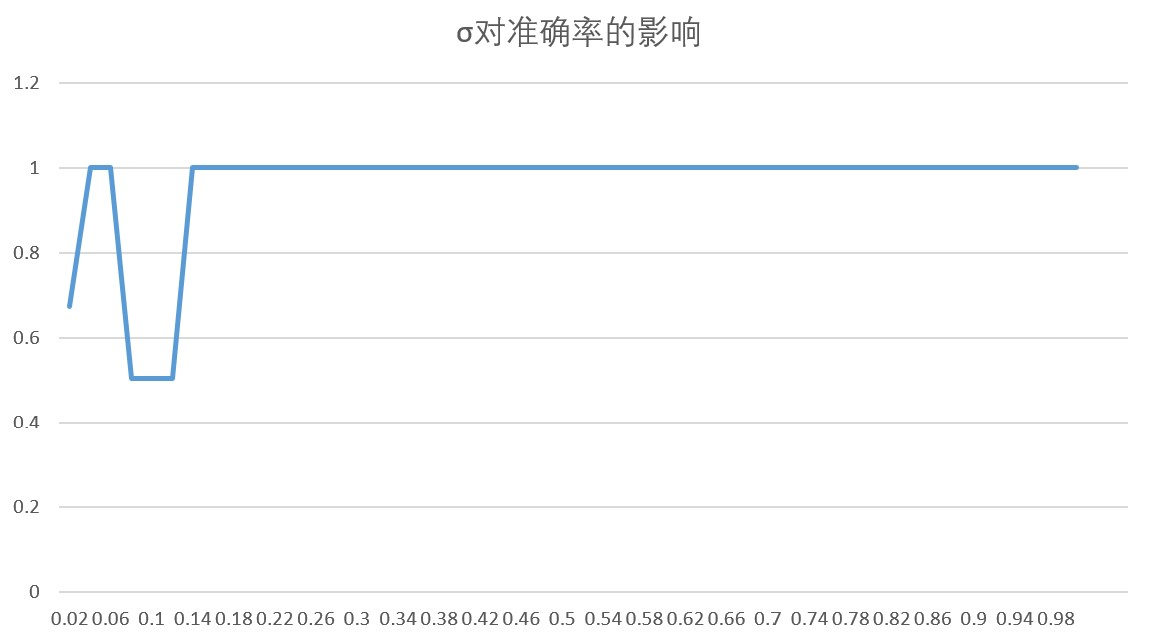
\includegraphics[width=3in]{2_1.jpg}
		\end{minipage}
	}
	\subfigure{
		\begin{minipage}[t]{0.45\linewidth}
			\centering
			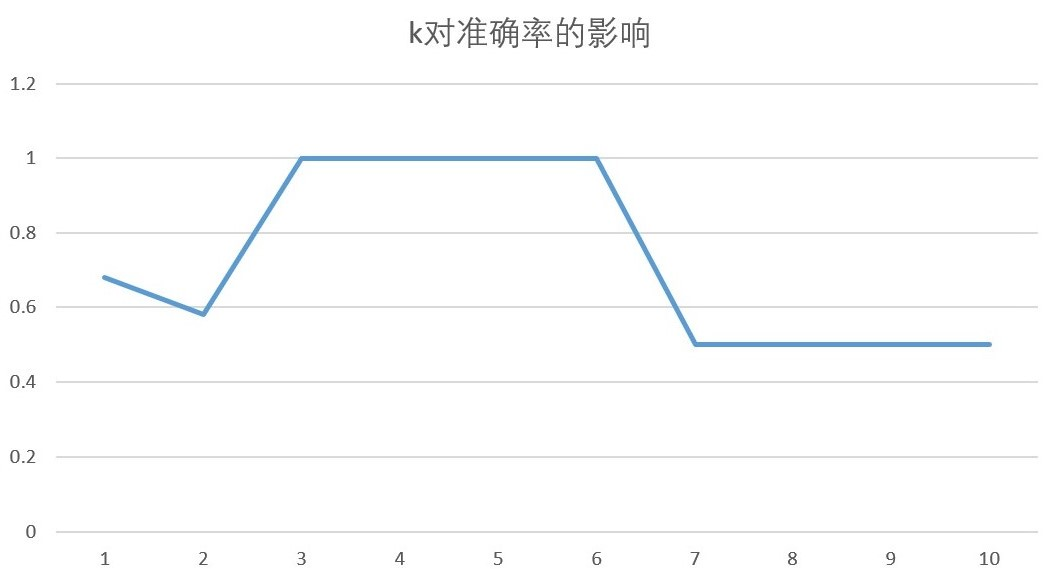
\includegraphics[width=3in]{2_2.jpg}
		\end{minipage}
	}
	\centering
	\caption{谱聚类中参数对准确率的影响}
	\label{figl}
\end{figure}

\end{document}
